\documentclass[conference]{IEEEtran}
\IEEEoverridecommandlockouts
% The preceding line is only needed to identify funding in the first footnote. If that is unneeded, please comment it out.
\usepackage{cite}
\usepackage{amsmath,amssymb,amsfonts}
\usepackage{algorithmic}
\usepackage{graphicx}
\usepackage{textcomp}
\usepackage{xcolor}
\usepackage{algorithm}
\def\BibTeX{{\rm B\kern-.05em{\sc i\kern-.025em b}\kern-.08em
    T\kern-.1667em\lower.7ex\hbox{E}\kern-.125emX}}
\begin{document}

\title {An Analysis of Government ID’s Implemented using NFTs \\[1ex] \large https://github.com/abdullahsalous/An-analysis-of-Government-ID-s-implemented-using-NFTs \\[1ex] \large https://youtu.be/JBvHuTlGf3Q}

\author{\IEEEauthorblockN{Abdullah Salous}
\IEEEauthorblockA{\textit{Computer Science} \\
\textit{University of Oklahoma}\\
Norman, United States \\
abdullah.r.salous-1@ou.edu}
}

\maketitle

\begin{abstract}
In the United States, traditional government-issued IDs such as driver's licenses, Social Security numbers, and passports are increasingly vulnerable to fraud, forgery, and data misuse. As a potential alternative, this paper explores the feasibility of a blockchain-based digital identification system using non-fungible tokens (NFTs). While the concept of on-chain identity is still emerging, several real-world implementations such as Proof of Humanity offer foundational insights. This study empirically analyzes these existing Web3 identity projects to identify their strengths, limitations, and technical design patterns. Additionally, the paper proposes a prototype schema for blockchain-based identity credentials. The proposed approach will be compared against current U.S. ID systems, focusing on security. The goal is to determine whether identity NFTs can practically enhance or complement national identity infrastructure in an effective way.
\end{abstract}

\section{Introduction}
In the age of technology, identity theft is an increasing and pertinent issue to many Americans. According to the Bureau of Justice Statistics, approximately 23.9 million U.S. residents aged 16 or older (9\% of the population) experienced identity theft in 2021, while nearly 1 in 5 adults reported having been victims at some point in their lives \cite{Bureau of Justice Statistics}. As illustrated in Figure \ref{fig:ID Theft}, data from the Federal Trade Commission shows a steady rise in reports of fraud, identity theft, and related issues over the past five years, with a significant spike in 2021. On average, identity theft alone accounts for approximately 300,000 reports each year. These incidents often involve the misuse of personal information such as Social Security numbers, driver's licenses, and bank details, leading to financial loss, legal complications, and long-term reputational damage. 

\begin{figure}[h!]
    \centering
    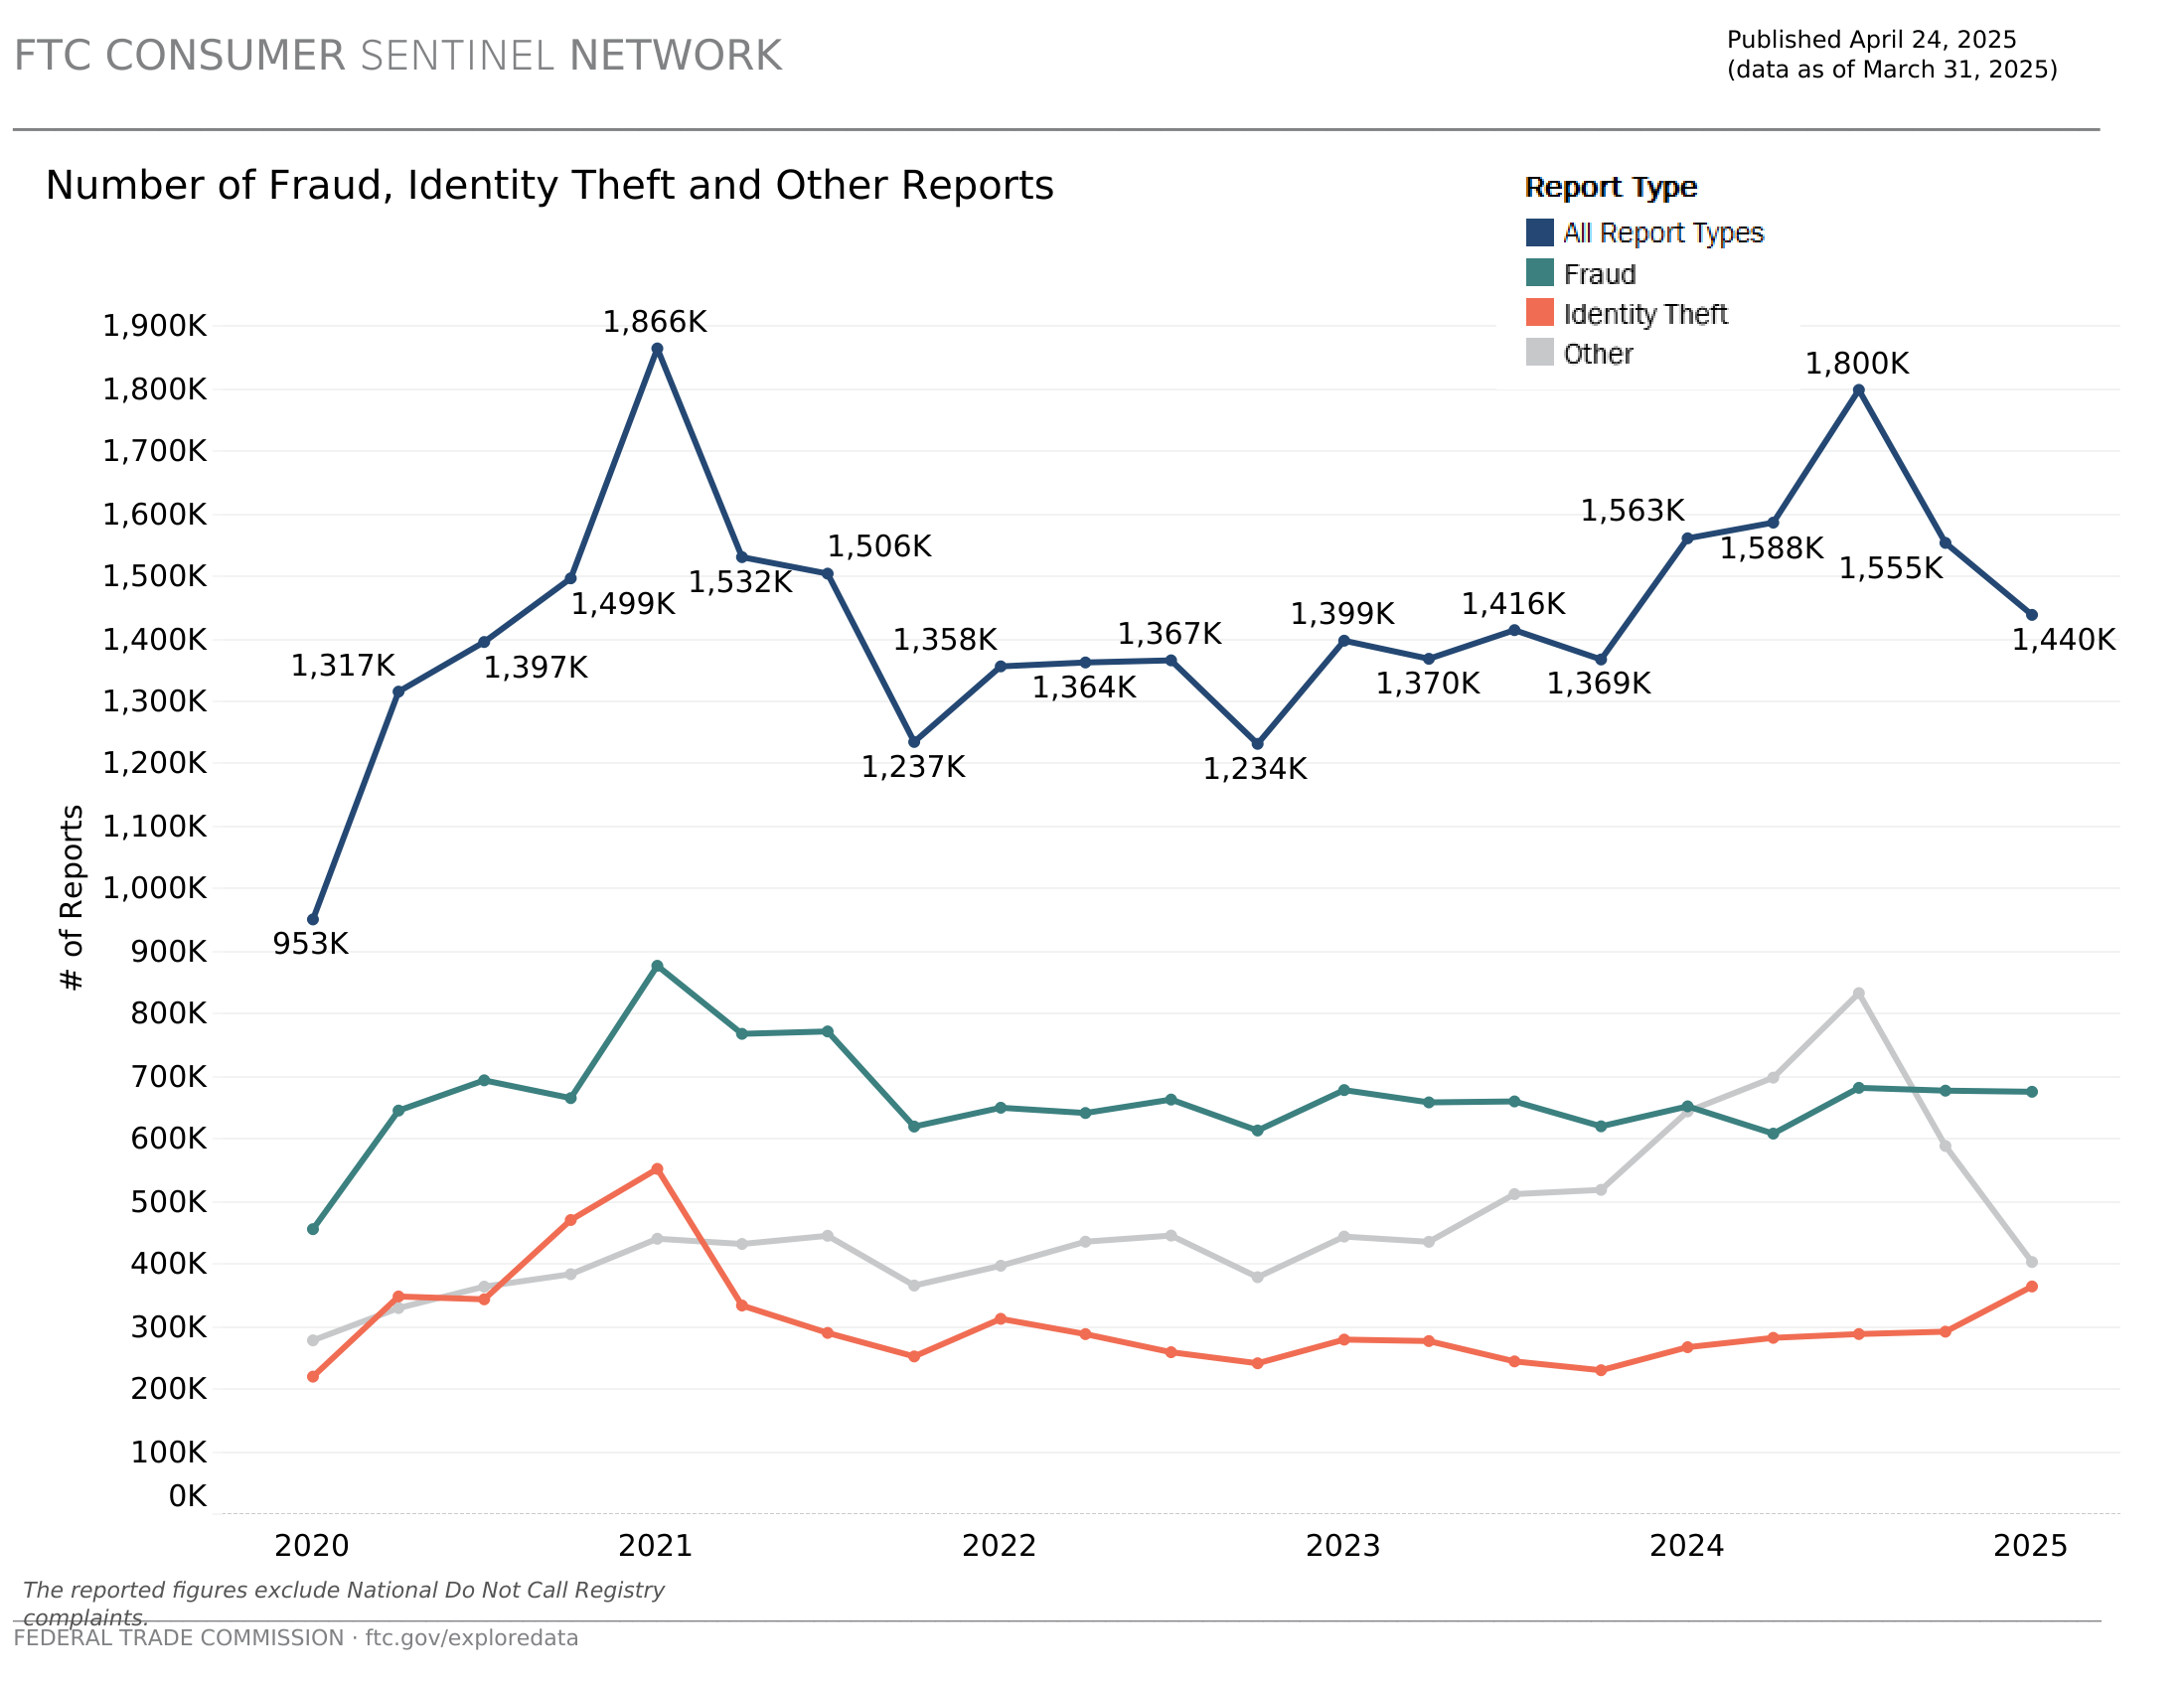
\includegraphics[width=0.9\linewidth]{Trends Over Time.png}
    \caption{Fraud, Identity Theft, and Other Reports}
    \label{fig:ID Theft}
\end{figure}

Despite the increasing sophistication of cybersecurity tools, traditional government-issued forms of identification remain vulnerable to theft, forgery, and data breaches. One significant concern is the widespread use of fake IDs, which are commonly used not only by underage individuals for age-restricted purchases, but also by criminals for more serious offenses such as identity fraud, illegal immigration, and financial scams. According to "IDScan.net", a study conducted found that 12.5\% of high school students admitted to possess a fake ID, and 32.2\% of college students under 21 admitted to possess it as well \cite{fake ID's}. As of 2024, CBS News reported that approximately 40,000 migrants from South and Central America entered the U.S. without authorization, with many resorting to purchasing counterfeit identification documents as a means of securing work to support their families \cite{cbs-news}. This shows the ease with which physical documents like driver's licenses or passports can be counterfeited or altered, thus highlights the limitations of document-based verification. Additionally, centralized identity repositories have proven to be high-value targets for cyberattacks. For instance, the 2015 breach of the U.S. Office of Personnel Management (OPM) compromised the personal data of over 21.5 million people \cite{opm}. These vulnerabilities expose structural weaknesses in existing systems and underscore the urgent need for more tamper-resistant, secure, and verifiable methods of identity management.

Blockchain technology, particularly through the use of non-fungible tokens (NFTs) presents a compelling alternative. These systems offer the promise of tamper-proof, self-sovereign digital identity that can be cryptographically verified and selectively disclosed by users. Several projects have begun experimenting with this concept, including various implementations of Proof of Humanity, each offering a different take on how identity can be established and managed on-chain.

Despite these innovations, the integration of blockchain-based identity into national systems like that of the U.S. remains largely unexplored. This paper investigates whether NFT-based identity systems built on platforms like Ethereum could provide a more secure and privacy-preserving framework for digital identification. By comparing blockchain-based identity models to current U.S. government systems, and by analyzing Etheruem's architecture, this study aims to evaluate the feasibility of adopting such technology at scale.


\section{Background \& Related Work}
The internet is rapidly evolving with the emergence of Web3, a new phase defined by decentralization, user ownership, and cryptographic security. Unlike the current Web2 landscape, where user data is controlled by centralized platforms, Web3 empowers individuals to manage their own identities and digital assets without relying on third parties \cite{what-is-web3}. This shift introduces new possibilities for privacy-preserving and tamper-resistant identity systems. Several projects, such as various implementations of Proof of Humanity are already exploring how decentralized technologies can reshape how we approach identity authentication.

\subsection{Decentralization}
When discussing any system, it is important to understand the system and the environment that surrounds it. Web3 technology shifts away from centralization, and hierarchical distribution, to a decentralized system. A decentralized system is a system where components operate on local information to achieve goals, rather than the result of a central ordering influence. This removes the need for a system to rely on a centralized authority and thus can unleash enormous potential in the space of identity verification. Centralized ID systems, create single points of failure which makes them vulnerable to data breaches, censorship, or misuse of authority. Figure \ref{fig:decentralized} helps visualize the difference between the various existing systems and the theoretical fault tolerance of a decentralized system.

\begin{figure}[h!]
    \centering
    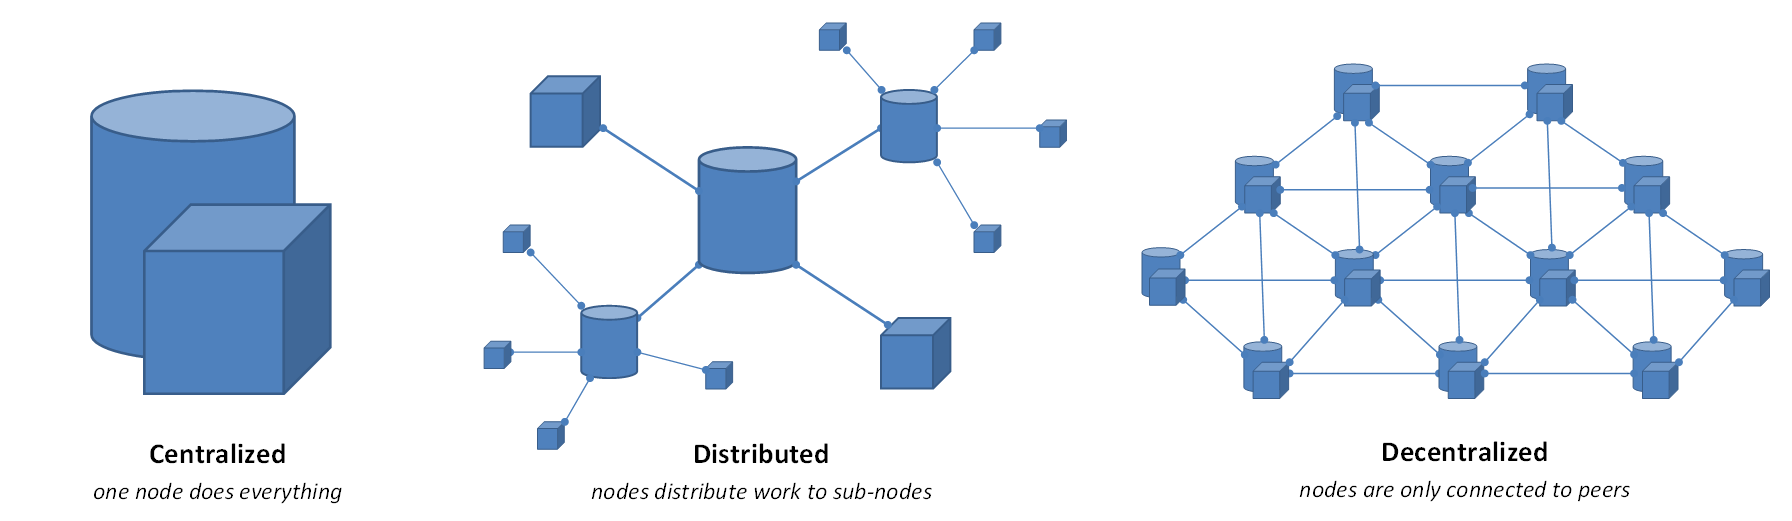
\includegraphics[width=0.9\linewidth]{decentralized.png}
    \caption{Centralized, Distributed, and Decentralized Systems | Ethereum Stack Exchange}
    \label{fig:decentralized}
\end{figure}

\subsection{Blockchain}
A blockchain is a data structure that is analogous to an append-only linked list. This ledger is distrubuted to form a distributed system. Additionally, adding to the ledger is done without a central authority using a consensus mechanism, which ensures agreement across the network on the validity of new transactions. In Ethereum’s case, this consensus is maintained by validators, who propose and attest to new blocks in exchange for rewards, thereby securing the network. Ethereum is a blockchain with a computer embedded in it. This system was revolutionary in that it was the first platform to introduce the concept of smart contracts. Smart contracts are programs uploaded and executed by the network. These programs are executed in a quasi–Turing complete programming environment by using gas to ensure that a program halts. The Ethereum Virtual Machine (EVM) maintains a consistent world state across all nodes in the network. The relationship between the execution and consensus client are highlighted in Figure \ref{fig:con-exe}. There are two types of accounts defined by Ethereum: externally owned accounts (EOAs) controlled by private keys, and contract accounts; which are governed by smart contract code. In our case, this can allow users to interact with smart contracts to register, verify, and manage digital identities without the need for a centralized entity. 

\begin{figure}[h!]
    \centering
    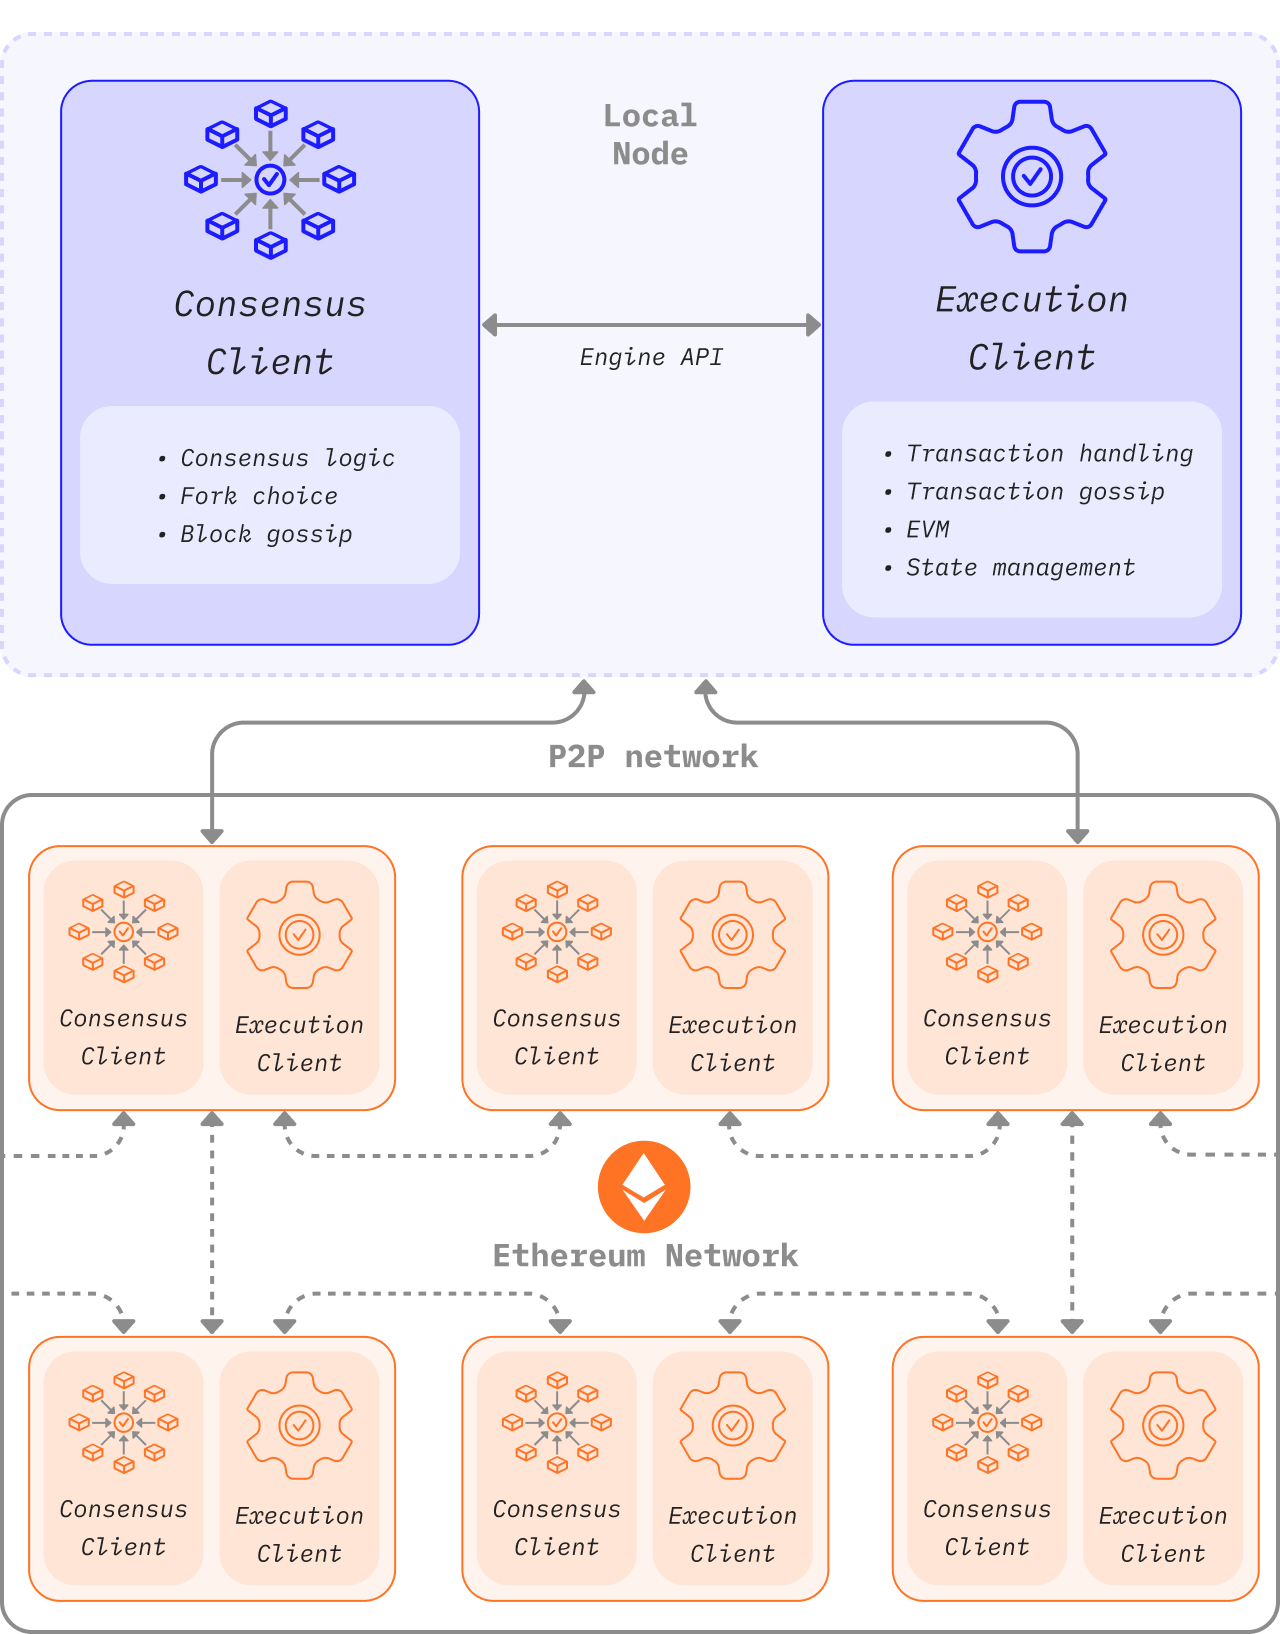
\includegraphics[width=0.9\linewidth]{consensus-execution.png}
    \caption{Ethereum Network Architecture | geth.ethereum.org}
    \label{fig:con-exe}
\end{figure}

\subsection{NFTs}
NFTs (non-fungible tokens) are unique digital assets stored on the Ethereum blockchain. Unlike regular tokens like ETH or USDC, which are all identical and interchangeable (fungible), each NFT is one-of-a-kind with distinct properties. This uniqueness makes NFTs ideal for representing individual digital or real-world items like art, collectibles, proving your online identity, ticketing, or real estate. NFTs are created and managed through Ethereum smart contracts, which follow standards like ERC-721 or ERC-1155. These contracts assign ownership, generate unique IDs, and store metadata that describes what each NFT represents. Since all ownership and transaction history is recorded on the blockchain, anyone can verify who owns a particular NFT. Additionally, NFT creators can program features like supply limits or automatic royalties into the smart contract, giving them more control and flexibility \cite{what-is-nft}. An example of this is shown in Figure \ref{fig:nft-exp}. As shown, the item is an image with "Blur: Blend" as the owner. The token standard is ERC-721 and the image is stored off-chain. It also shows the creator (address that deployed the smart contract) of the NFT and additional properties of the item. 

\begin{figure}[h!]
    \centering
    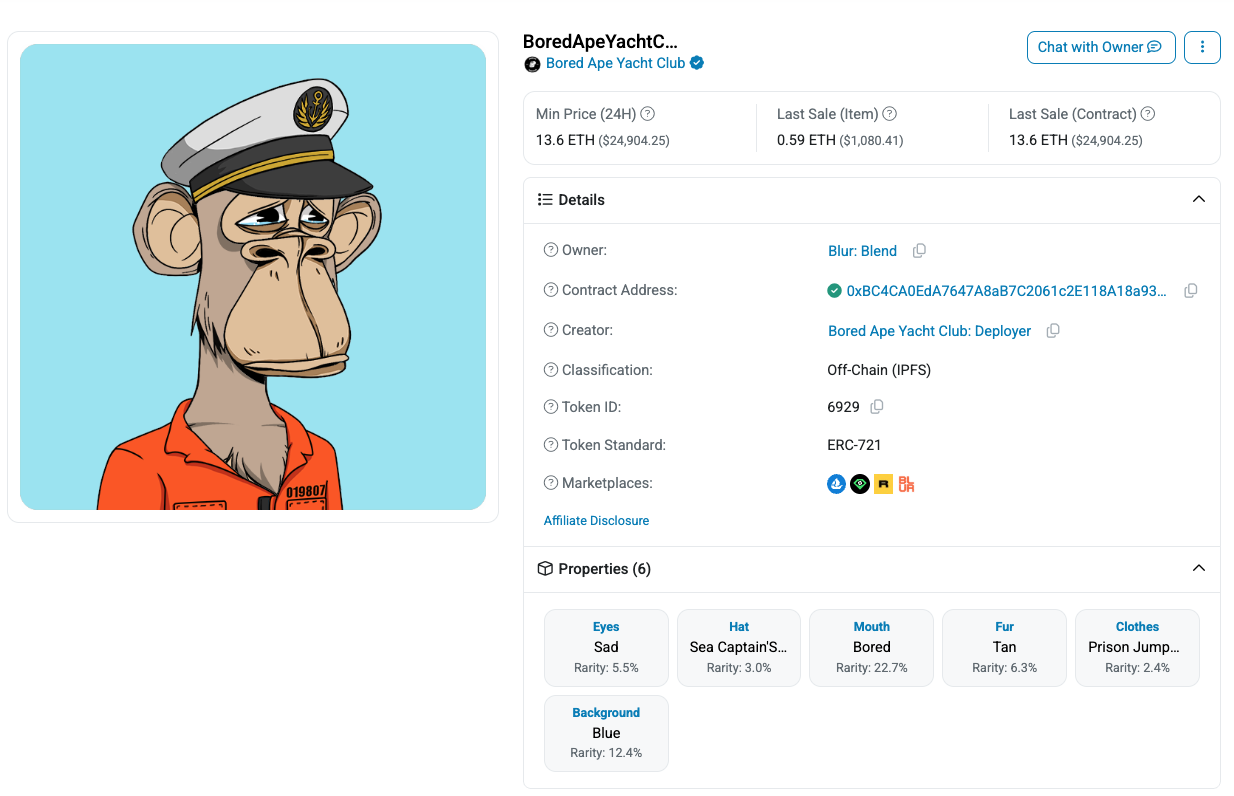
\includegraphics[width=0.9\linewidth]{nft-example.png}
    \caption{Example NFT | etherscan.io}
    \label{fig:nft-exp}
\end{figure}

\subsection{Proof of Humanity}
Proof of Humanity (PoH) is a decentralized identity verification system designed to ensure that participants in a digital ecosystem are real, human individuals rather than bots \cite{what-is-poh}. As artificial intelligence grows increasingly capable of mimicking human behavior and speech, the need for reliable human verification has become more urgent. Proof of Humanity addresses this challenge by combining social verification with a reputation-based system on the Ethereum blockchain. There are many different implementations of Proof of Humanity. In this paper, we will focus on Proof of Humanity by Kleros.

The first implementation to examine is Proof of Humanity by Kleros. PoH by Kleros requires users to first connect an online wallet. The wallet address provided by the user is publicly linked to their identity. Then, the registration process begins. Registration requires a user to submit a name, photo, and video holding their wallet address. They are then vouched for by an existing verified member as shown in Figure \ref{fig:poh-kleros}. This crowd-sourced, tamper-resistant approach can reduce the risk of Sybil attacks and fake accounts while giving users greater control over their online interactions. By removing the need for centralized authorities, Proof of Humanity by Kleros seeks to offer a trustable and scalable framework for authenticating digital identity in Web3.

\begin{figure}[h!]
    \centering
    
\includegraphics[width=0.9\linewidth]{poh-kleros.png}
    \caption{Proof of Humanity Registration}
    \label{fig:poh-kleros}
\end{figure}

What sets Proof of Humanity apart is its use of a Humanity ID. This is a unique identifier tied to each human rather than to a private key or wallet as shown in Figure \ref{fig:poh-humanity-id}. The Humanity ID remains constant even if the wallet address changes, ensuring that the system verifies the person, not just their device. All valid identities across multiple chains are compiled into a unified registry, with one active home chain per ID. The registration criteria include the submitter being alive, not previously registered, and must provide clear and accurate evidence, such as a video showing internal facial features and the wallet address. Proof of Humanity by Kleros does not use a traditional NFT implementation \cite{poh-policy}.

\begin{figure}[h!]
    \centering
    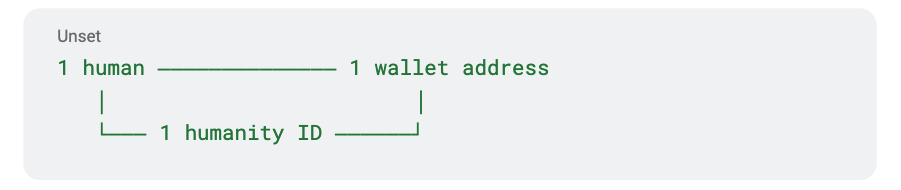
\includegraphics[width=0.9\linewidth]{poh-humanity-id.png}
    \caption{Humanity ID}
    \label{fig:poh-humanity-id}
\end{figure}

The system also allows users to challenge pending submissions based on various criteria. These include Sybil attacks (duplicate or fake registrations), identity theft, and incorrect or incomplete submissions. Additionally, deceased individuals can be removed if verifiable evidence is provided. If challenged, registrants must provide proof such as a video reading a recent block hash to remain in the registry \cite{poh-policy}.

\subsection{Other Implementations}
Another implementation of identity verification is Polygon ID. Polygon ID is a digital identity platform that uses zero-knowledge cryptography to give users full control over their identity while preserving privacy. Polygon ID is the first identity solution that is private-by-default, and capable of secure on-chain verification. Unlike traditional digital IDs or NFT-based credentials, Polygon ID uses zero-knowledge proofs to let users prove things about themselves without revealing the underlying data. The system is powered by the Iden3 protocol and Circom ZK toolkit, and supports a new model where users can issue and receive attestations without needing a third party. These claims are flexible, composable, and more expressive than NFTs or Verifiable Credentials (VCs), which often fall short on privacy and scalability \cite{polygon}.

\section{Comparative Analysis}

\subsection{Benefits and Drawbacks of NFT-based Approaches}
NFT-based identity systems offer a verifiable, tamper-evident way to link identities and blockchain records. The immutability of NFTs helps ensure the authenticity of issued credentials. However, these benefits come at the cost of privacy, as NFT metadata is often stored publicly and can be easily linked to wallets, leading to de-anonymization. Additionally, minting NFTs incurs gas fees, which can limit scalability and accessibility, especially on high-cost networks like Ethereum. NFTs also struggle with revocability, since once an NFT is minted, it is permanently on the blockchain. If someone loses eligibility of an attribute, the NFT cannot be unilaterally revoked by the issuer.

\subsection{Comparison between Proof of Humanity \& Polygon ID}
Proof of Humanity and Polygon ID have their unique approaches to verifying identity. Proof of Humanity relies on community-based verification where users submit a video, name, and photo and must be vouched for by others. This system is tamper-resistant because it makes it difficult for bots or fake identities to get through. Polygon ID is also tamper-resistant but uses zero-knowledge cryptography instead of social validation. This means it can mathematically prove someone meets certain criteria without revealing any personal information. Privacy is one of the biggest differences between the two. Proof of Humanity is very public by design. An individual's video and wallet address are available on-chain for anyone to see. This transparency increases trust but sacrifices privacy. Polygon ID, on the other hand, is private by default. It uses zero-knowledge proofs to let users prove things about themselves such as being over 18 without ever sharing their name, birth date, or other details. This makes Polygon ID much better suited for privacy-sensitive use cases.

\section{Prototype Schema Design}
Government ID's typically have specific characteristics. These include a photo and other important information such as an address and an individual's physical characteristics. They also include a unique identification number to be able to authenticate the validity of the ID. It is important for a Government ID to allow some of these characteristics to be updated such as height, weight etc. It is also equally important for Government ID's to be revocable. To modernize the U.S. identity system with privacy, programmability, and decentralization in mind, we propose a blockchain-based prototype identity framework using the Ethereum network. In this design, identity credentials are issued by trusted government agencies in the form of digitally signed Verifiable Credentials. These credentials are not stored on-chain but are cryptographically hashed and anchored to Ethereum for tamper-evident verification and revocation tracking. Users store their credentials in their wallets on their personal devices which enables them to disclose only necessary identity traits when interacting with verifiers, such as banks or airports.

A fundamental feature of this system is its use of zero-knowledge proofs. Zero-knowledge are cryptographic methods that allow one party (the prover) to demonstrate to another party (the verifier) that a given statement is true without revealing any information beyond the validity of that statement. For example, a user could prove they are over 18 years old without revealing their exact date of birth, or prove U.S. citizenship without disclosing their name or address. These proofs are constructed using protocols like zkSNARKs (from Polygon ID) and validated off-chain while referencing on-chain attestations. This ensures user privacy when sharing information. Each Verifiable Credential is issued alongside a revocation mechanism. If a credential is expired or updated, the issuing agency can revoke or reissue the credential by updating the on-chain registry. This preserves the flexibility required in government identification. As mentioned previously, one of the downsides to NFTs is the fact that they are difficult to revoke and do not maintain privacy. Therefore, the zero-knowldege proof schema similar to Polygon ID's is most compatible with Government ID implementation.

\section{Conclusion}
In summary, we compared two blockchain‐based ID systems, Proof of Humanity by Kleros, which uses community vetting but makes personal data public, and Polygon ID, which keeps data private through zero‐knowledge proofs but requires more complex cryptography. We then outlined a U.S. government prototype that issues digitally signed credentials anchored on Ethereum. Under this design, citizens hold their own credentials in personal wallets, use zero‐knowledge proofs to share only the needed information, and rely on an on‐chain registry to revoke or update IDs without exposing private details. Next steps are to build and test a working demo, and test for security, usability, and legal compliance.

\begin{thebibliography}{00}
\bibitem{Bureau of Justice Statistics}“Victims of identity theft, 2021,” Bureau of Justice Statistics, https://bjs.ojp.gov/press-release/victims-identity-theft-2021. 

\bibitem{fake ID's}D. Papich, “How common are fake ids?,” IDScan.net,
https://idscan.net/blog/how-common-are-fake-ids/?srsltid=AfmBOoqOPSxNFDdifCClManqCJyKoqzAF2s6jpc2qWSBfe4UzCP-ylch

\bibitem{cbs-news}K. Weis, “Criminals selling fake identity documents to migrants in Colorado desperate to find work, CBS News Colorado Investigation finds,” CBS News, https://www.cbsnews.com/colorado/news/criminals-selling-fake-identity-documents-migrants-colorado-desperate-find-work-cbs-news-colorado-investigation-finds/. 

\bibitem{opm}J. Bracy, IAPP, https://iapp.org/news/a/21-5-million-breached-in-second-opm-hack. 

\bibitem{what-is-web3}P. Shoemaker, “What is web3? web 3.0 explained,” Identity, https://www.identity.com/web3/.

\bibitem{what-is-poh}P. Shoemaker, “Why proof of humanity is more important than ever,” Identity, https://www.identity.com/why-proof-of-humanity-is-more-important-than-ever/.

\bibitem{what-is-nft}“Non-fungible tokens (NFT),” ethereum.org, https://ethereum.org/en/nft/#nft-use-cases.

\bibitem{poh-policy}“Proof of Humanity Registry Policy,” Proof of humanity V2

\bibitem{polygon}Polygon Labs, “Introducing polygon ID, zero-knowledge identity for WEB3,” Polygon, https://polygon.technology/blog/introducing-polygon-id-zero-knowledge-own-your-identity-for-web3. 

\end{thebibliography}

\end{document}
